\section{Mô hình Linear Regression}
\subsection{Cài đặt và huấn luyện mô hình}

\subsubsection{Tiền xử lý dữ liệu}
\begin{itemize}
    \item \textbf{Đọc dữ liệu:} Từ file CSV phân cách bằng dấu `;`, chuẩn hoá dữ liệu kiểu châu Âu (dấu phẩy `,` chuyển thành chấm `.`).
    \item \textbf{Xử lý dữ liệu thiếu:} Giá trị \texttt{-200} được xem là thiếu và thay bằng \texttt{NaN}. Các cột toàn \texttt{NaN} hoặc không hợp lệ (\texttt{Unnamed}) bị loại bỏ.
    \item \textbf{Biến thời gian:} Kết hợp \texttt{Date} và \texttt{Time} thành \texttt{DateTime}, sau đó trích xuất thêm các đặc trưng \texttt{Hour}, \texttt{Day}, \texttt{Month}, \texttt{DayOfWeek}.
\end{itemize}

\subsubsection{Xử lý đặc trưng}
\begin{itemize}
    \item Loại bỏ các cột không phải kiểu số hoặc không còn cần thiết.
    \item Loại bỏ các hàng có \texttt{NaN} trong biến mục tiêu \texttt{CO(GT)}.
    \item Sử dụng \texttt{KNNImputer} để xử lý giá trị thiếu trong tập đặc trưng.
\end{itemize}

\subsubsection{Kỹ thuật mở rộng đặc trưng (Feature Engineering)}
\begin{itemize}
    \item Tạo thêm 3 đặc trưng phi tuyến:
    \begin{itemize}
        \item \texttt{PT08.S1(CO)} $\times$ \texttt{NOx(GT)}
        \item \texttt{PT08.S5(O3)}$^2$
        \item \texttt{NO2(GT)} $\times$ \texttt{RH}
    \end{itemize}
\end{itemize}

\subsubsection{Xử lý ngoại lệ (Outliers)}
\begin{itemize}
    \item Sử dụng phương pháp IQR để loại bỏ outliers ở cả tập đặc trưng và mục tiêu.
\end{itemize}

\subsubsection{Chia dữ liệu}
\begin{itemize}
    \item Chia dữ liệu thành tập huấn luyện (80\%) và tập kiểm thử (20\%).
    \item Chuẩn hóa dữ liệu bằng \texttt{StandardScaler}.
\end{itemize}

\subsubsection{Huấn luyện mô hình}
\begin{itemize}
    \item Sử dụng mô hình \textbf{Linear Regression với ràng buộc hệ số không âm} (\texttt{positive=True}) để đảm bảo các đặc trưng không có tác động âm tới \texttt{CO(GT)}.
    \item Mô hình được huấn luyện trên tập huấn luyện đã chuẩn hóa.
\end{itemize}

\subsection{Tuning Hyperparameters}

\subsubsection{Đặc điểm}
\begin{itemize}
    \item Linear Regression không có quá nhiều siêu tham số. Trong code, có sử dụng:
    \begin{itemize}
        \item \texttt{positive=True}: Ép các hệ số của mô hình phải lớn hơn hoặc bằng 0, phù hợp với các đặc trưng vật lý như nồng độ khí, độ ẩm, v.v.
    \end{itemize}
\end{itemize}

\subsubsection{Chiến lược tối ưu hoá gián tiếp}
\begin{itemize}
    \item Tối ưu chất lượng dữ liệu đầu vào thông qua:
    \begin{itemize}
        \item Xử lý giá trị thiếu bằng \texttt{KNNImputer}.
        \item Loại bỏ outliers với IQR.
        \item Thêm đặc trưng phi tuyến $\Rightarrow$ giúp mô hình tuyến tính mô tả tốt hơn mối quan hệ phi tuyến.
    \end{itemize}
\end{itemize}

\noindent \textit{\textbf{Lưu ý:}} Không sử dụng \texttt{GridSearchCV} hay \texttt{Cross-Validation}, do mô hình đơn giản và quá trình tối ưu tập trung vào xử lý dữ liệu đầu vào.

\subsection{Kết quả và đánh giá}

\subsubsection{Đánh giá trên tập kiểm thử}
\begin{itemize}
    \item \textbf{Mean Squared Error (MSE):} 0.0972
    \item \textbf{Root MSE (RMSE):} 0.3118
    \item \textbf{Mean Absolute Error (MAE):} 0.2088
    \item \textbf{R\textsuperscript{2} score:} 0.8673 $\Rightarrow$ mô hình giải thích khoảng 86.73\% phương sai của dữ liệu.
\end{itemize}

\subsubsection{Diễn giải hệ số}
\begin{itemize}
    \item Các hệ số được trích xuất và sắp xếp theo mức độ ảnh hưởng.
    \item \textbf{Top 5 đặc trưng ảnh hưởng mạnh nhất (theo trị tuyệt đối hệ số):}
\end{itemize}

\begin{center}
\begin{tabular}{|l|c|}
\hline
\textbf{Feature} & \textbf{Coefficient} \\
\hline
C6H6(GT) & 0.576522 \\
PT08.S1(CO) & 0.151165 \\
PT08.S3(NOx) & 0.127041 \\
NOx(GT) & 0.126015 \\
NO2(GT) & 0.069689 \\
\hline
\end{tabular}
\end{center}

\subsubsection{Biểu đồ trực quan}
\begin{itemize}
    \item So sánh giá trị dự đoán và thực tế.
    \begin{figure}[H]
        \centering
        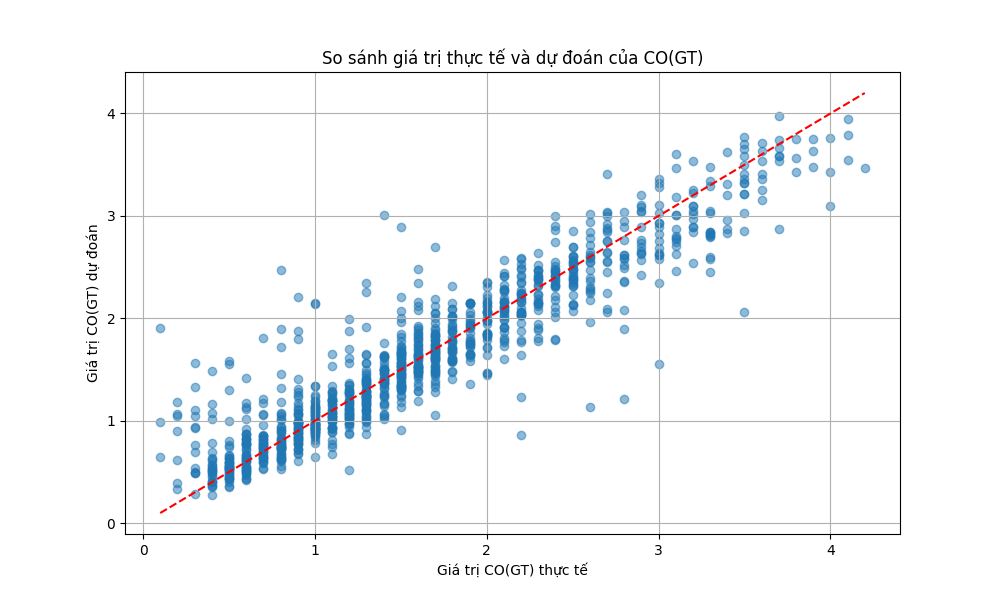
\includegraphics[width=0.65\textwidth]{images/Linear_regression/actual_vs_predicted.png}
        \caption{So sánh giá trị dự đoán và thực tế}
        \label{fig:importance}
    \end{figure}
    \item Phân phối và phân tán sai số.
    \begin{figure}[H]
        \centering
        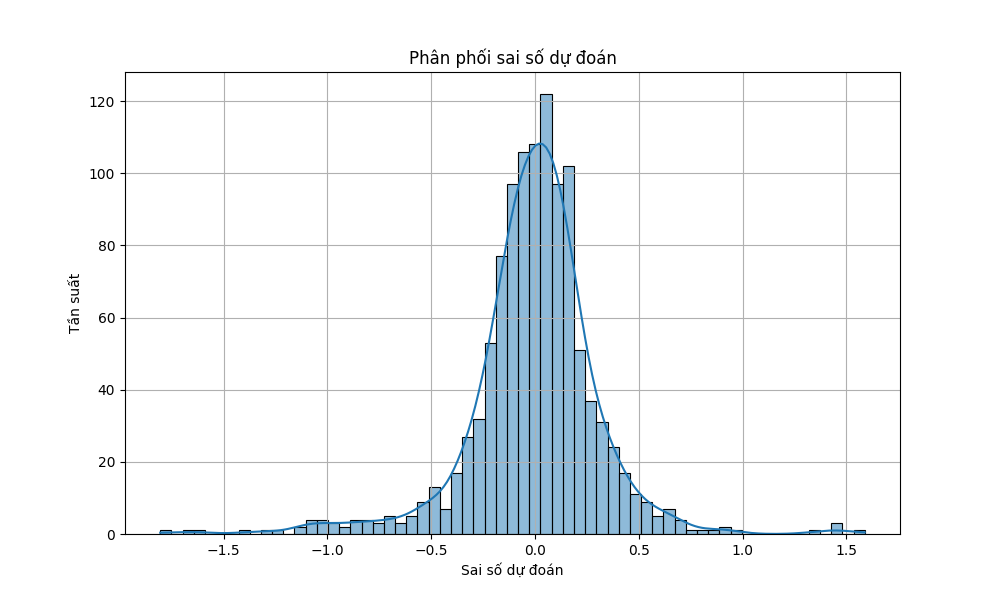
\includegraphics[width=0.9\textwidth]{images/Linear_regression/residuals_histogram.png}
        \caption{Phân phối sai số dự đoán}
        \label{fig:importance}
    \end{figure}
    \begin{figure}[H]
        \centering
        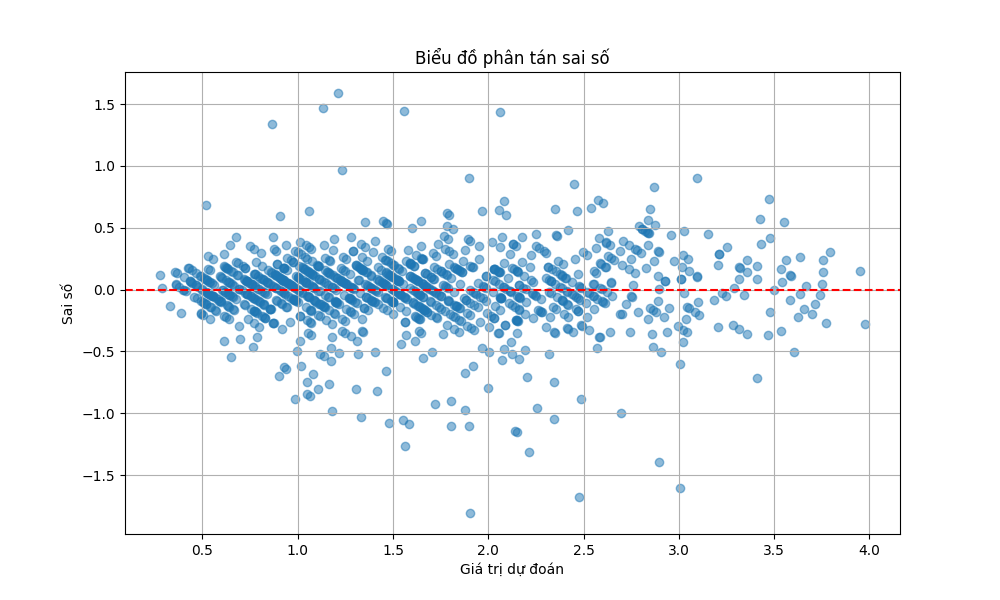
\includegraphics[width=0.9\textwidth]{images/Linear_regression/residuals_scatter.png}
        \caption{Biểu đồ phân tán sai số}
        \label{fig:importance}
    \end{figure}
    \item Mức độ quan trọng của các đặc trưng.
    \begin{figure}[H]
        \centering
        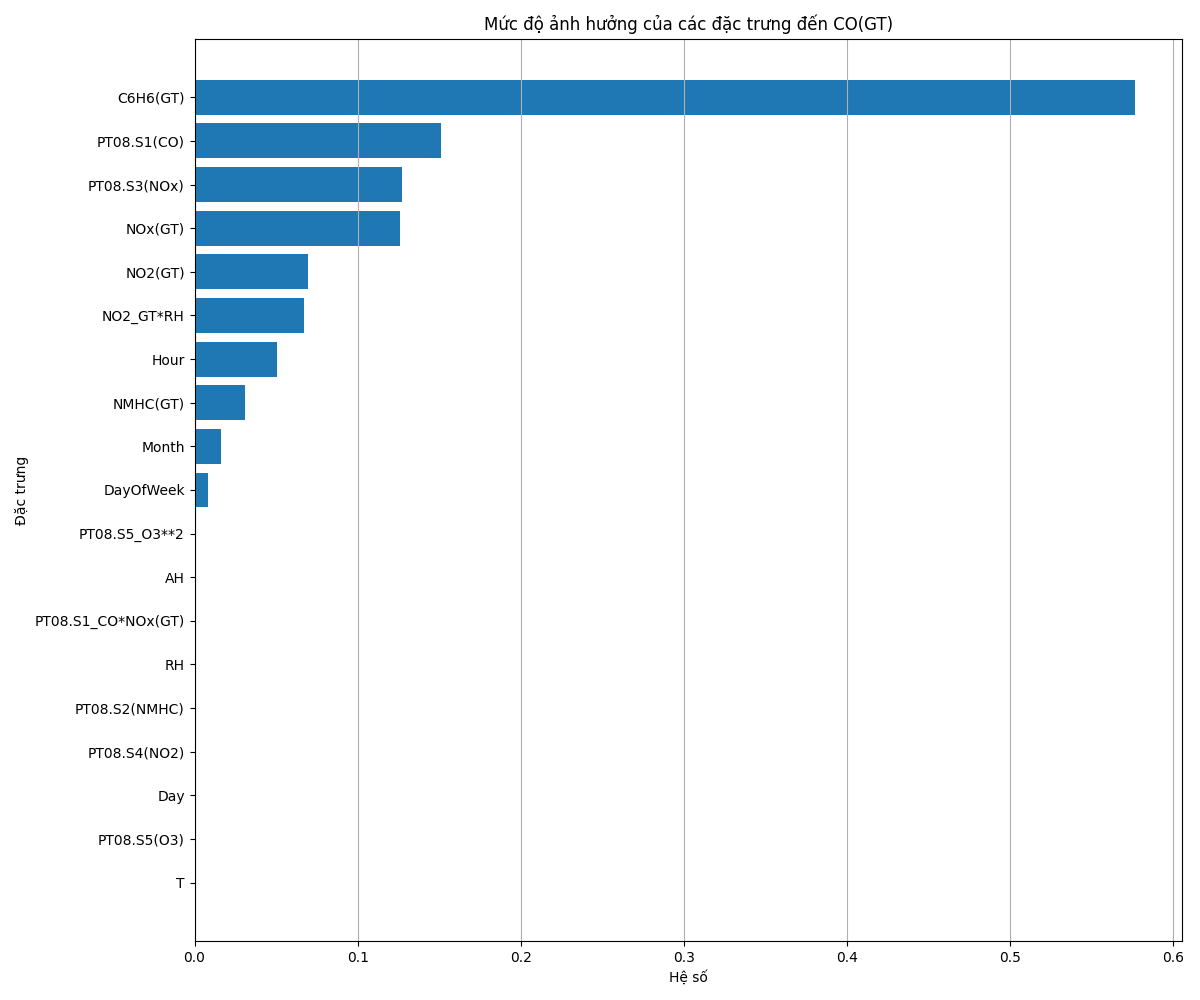
\includegraphics[width=0.9\textwidth]{images/Linear_regression/feature_importance.png}
        \caption{Tầm quan trọng của các đặc trưng}
        \label{fig:importance}
    \end{figure}
\end{itemize}

\subsubsection{Dự đoán thử và kiểm tra sai số}
\begin{itemize}
    \item Thử dự đoán 5 dòng từ tập kiểm thử và in sai số từng dòng.
    \item Sai số trung bình: \textbf{0.2110}, cho thấy độ chệch không quá lớn.
\end{itemize}

\subsection{Kết luận}
Mô hình Linear Regression đã được triển khai thành công với quy trình xử lý dữ liệu kỹ lưỡng và các kỹ thuật feature engineering phù hợp. Mô hình đạt được độ chính xác đáng kể với \textbf{R² = 86.73\%}, phản ánh mối quan hệ tuyến tính mạnh mẽ giữa các đặc trưng và biến mục tiêu. Các đặc trưng được lựa chọn và chuẩn hóa đã góp phần quan trọng trong việc nâng cao hiệu suất dự đoán. Kết quả này cho thấy mô hình\textbf{ Linear Regression} là một lựa chọn hiệu quả và dễ diễn giải cho bài toán dự đoán này.
